\documentclass{article}
\usepackage[margin=1in]{geometry}
\usepackage{amsmath, amssymb, tikz, pgfplots}
\usetikzlibrary{positioning}

\title{\vspace{-3ex}Advanced Function Notes}
\author{Jeffrey Gao\and More Contributors Later}
\renewcommand\thesubsubsection{\thesubsection{} \Alph{subsubsection}}
\renewcommand\labelitemi{--}

\begin{document}
	\maketitle
	
	\section{Unit 1}
	\subsection{Functions}
	\subsubsection{Relations}
	A (binary) relation is defined as a set of ordered pairs $(x, y)$. A relation can be described using:
	\begin{itemize}
		\item words
		\item graphs
		\item equations
		\item inequalities
		\item lists of ordered pairs
		\item mapping diagrams
	\end{itemize}
	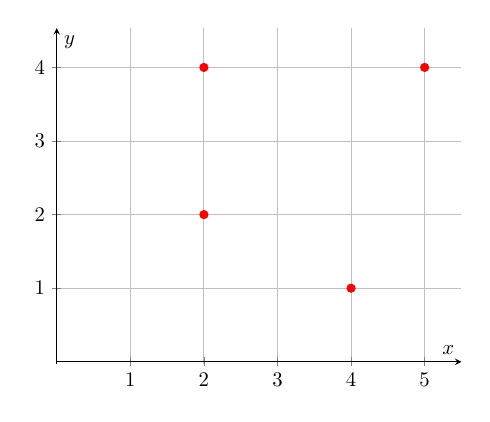
\begin{tikzpicture}[scale=.75]
		\begin{axis}[
			scatter/classes={a={draw=red,fill=red}},
			axis y line*=left,
			axis x line*=bottom,
			grid=both,
			ymin=0,
			xmin=0,
			ymax=4.5,
			xmax=5.5,
			axis equal,
			axis lines=middle,
			xlabel=$x$,
			ylabel=$y$,
			xtick distance=1,
			ytick distance=1
		]
		\addplot[scatter,only marks,scatter src=explicit symbolic]
		table[meta=label] {
			x y label
			2 2 a
			2 4 a
			4 1 a
			5 4 a
		};
		\end{axis}
	\end{tikzpicture}\\
	This relation as a set of ordered pairs is $R=\{(2, 2), (2, 4), (4, 1),(5, 4)\}$
	\subsubsection{Domain and Range of a Function}
	The domain of a relation is the set of all the x values such that the ordered pair $(x, y)$ satisfies (is an element of) the relation. The range of a relation is the set of all the y values such that the ordered pair $(x, y)$ satisfies (is an element of) the relation.\\\\
	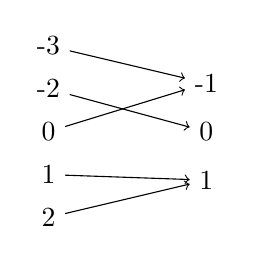
\begin{tikzpicture}[scale=.5]
		\node (n3) {-3};
		\node[below=2pt of n3] (n2) {-2};
		\node[below=2pt of n2] (o) {0};
		\node[below=2pt of o] (p1) {1};
		\node[below=2pt of p1] (p2) {2};
		
		\node[right=45pt of o] (o2) {0};
		\node[above=4pt of o2] (nn1) {-1};
		\node[below=4pt of o2] (pp1) {1};
		
		\draw[->] (n3) -- (nn1);
		\draw[->] (n2) -- (o2);
		\draw[->] (o) -- (nn1);
		\draw[->] (p1) -- (pp1);
		\draw[->] (p2) -- (pp1);
	\end{tikzpicture}
	For this mapping diagram, the domain would be $D=\{-3, -2, 0, 1, 2\}$ and the range would be $R=\{-1, 0, 1\}$
	\subsubsection{Functions}
	A function can only assign one element from the set of Y values (the range) to each element from the set of X values (the domain). $y=f(x)$ where $x$ is the argument or the input of the function and $y$ is the value or the output of the function.\\
	Using the function $f(x)=(x-1)^2$:
	\begin{itemize}
		\item $f(0)=1$
		\item $f(\frac{1}{2})=\frac{1}{4}$
		\item $f(a+2)=a^2+2a+1$
	\end{itemize}
	\subsubsection{Graph}
	The graph of a function $f$ is the graph of the set of ordered pairs $(x, y)$ where $y=f(x)$.\\
	The graph of the function defined by a set of ordered pairs $f=\{(2, 3), (0, -2), (-4, 3), (4, 0), (-3, -3)\}$:\\
	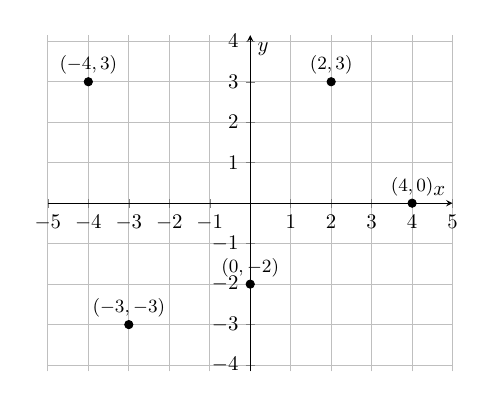
\begin{tikzpicture}[scale=.75]
		\begin{axis}[
			scatter/classes={a={draw=red,fill=red}},
			axis y line*=left,
			axis x line*=bottom,
			grid=both,
			ymin=-4,
			xmin=-5,
			ymax=4,
			xmax=5,
			axis equal,
			axis lines=middle,
			xlabel=$x$,
			ylabel=$y$,
			xtick distance=1,
			ytick distance=1
		]
		%TODO: Fix this so that the points are still red (Change the label something)
		\addplot[mark=*,scatter,only marks,scatter src=explicit symbolic,nodes near coords={\labelz}, visualization depends on={value {\small$(\thisrowno{0}, \thisrowno{1})$}\as\labelz}]
		table[meta=label] {
			x y label
			2 3 a
			0 -2 a
			-4 3 a
			4 0 a
			-3 -3 a
		};
		\end{axis}
	\end{tikzpicture}
	\subsubsection{Vertical Line Test}
	All functions are relations but not all relations are functions. A graph represents a function if every vertical line intersects the graph in at most one point.\\
	The set of ordered pairs $\{(0, 0), (-1, -1), (2, 2), (1, -1)\}$ represents a function, while the set of ordered pairs $\{(2, 3), (-1, 3), (2, -2), (-3, -1)\}$ does not.
	%TODO: The actual graphs with vertical lines
	\subsubsection{Domain and Range}
	The domain of a function $f$ is the set of all real numbers $x$ for which $f(x)$ is defined. The range of a function $f$ is the set of all real numbers $y$ for which $y=f(x)$  is defined.\\
	The domain and range for the set of ordered pairs $\{(-2, 0), (-1, 1), (0, -1), (1, 0)\}$ is $D=\{-2, -1, 0, 1\}$ and $\{-1, 0, 1\}$. The domain and range for the set of ordered pairs $\{(-1, 0), (0, 1), (1, 0), (3, 1), (7, 0)\}$ is $D=\{-1, 0, 1, 3, 7\}$ and $\{0, 1\}$.
	%TODO: Graphs with domain and range
	\subsubsection{Restrictions}
	Division by 0 is undefined, so the denominator of a function cannot equal 0. Square roots are undefined for negative numbers and square roots cannot be negative, so for $f(x)=\sqrt{x}$, $x\geq0$ and $f(x)\geq0$. Squares cannot be negative so for $f(x)=x^2$, $f(x)\geq0$.\\
	For $y=(x-1)^2-3$:
	\begin{itemize}
		\item $D=\{x\in R\}$
		\item $R=\{y\in R\mid y\geq-3\}$
	\end{itemize}
	For $y=2+\sqrt{x-3}$:
	\begin{itemize}
		\item $D=\{x\in R\mid x\geq3\}$
		\item $R=\{y\in R\mid y\geq2\}$
	\end{itemize}
	For $y=\frac{x-2}{x+2}$: $=\frac{x+2-4}{x+2}$ $=1-\frac{4}{x+2}$
	\begin{itemize}
		\item $D=\{x\in R\mid x\neq-2\}$
		\item $R=\{y\in R\mid y\neq1\}$
	\end{itemize}
	\subsection{Exploring Absolute Value}
	\subsubsection{Absolute Value}
	The absolute value $|x|$ of a real number $x$ is the distance between $x$ and 0.\\
	For example, $|5|=|-5|=5$ and $\left|2-\left|-3\right|\right|$.
	\subsubsection{Definition of Absolute Value}
	The absolute value $|x|$ is defined by:
	\[|x|=\begin{cases}
		x&\text{if }x\geq0\\
		-x&\text{if }x<0
	\end{cases}\]
	Therefore:
	\[|x-3|=\begin{cases}
		x-3&\text{if }x\geq3\\
		-x+3&\text{if }x<3
	\end{cases}\]
	\subsubsection{Properties of Absolute Value}
	Absolute values have the following properties:
	\begin{itemize}
		\item $|a|=|-a|$
		\item if $|a|=0$, $a=0$
		\item $|ab|=|a||b|$
		\item $\left|\frac{a}{b}\right|=\frac{|a|}{|b|}$
		\item $|a+b|\leq|a|+|b|$ (proved by triangle inequality)
	\end{itemize}
	For example, $\left|\frac{-2x}{3y}\right|\left|\frac{-2y}{3x}\right|=\frac{|-2||x|}{|3||y|}\cdot\frac{|-2||y|}{|3||x|}=\frac{4}{9}$. Also, $|-3x|-|-x|-|x|=3|x|-|x|-|x|=|x|$
	\subsubsection{Distance between two numbers}
	The distance between two numbers $a$ and $b$ on the number line can be represented by $|a-b|$.
	For example, in the equation $|x-3|=|5-x|$, $x$ would represent a number that is the same distance from 3 as is to 5. This can be solved algebraically:
	\begin{align*}
		&&x-3&=\pm(5-x)\\
		\text{Ca}&\text{se 1}&&&\text{Ca}&\text{se 2}\\
		x-3&=5-x&&&x-3&=x-5\\
		2x&=8&&&-3&=-5\\
		x&=4&&&\text{No }&\text{Solution}\\
		&&\therefore{}&x=4
	\end{align*}
	\subsubsection{Equations}
	If $E(x)$ is an algebraic expression containing the variable $x$, the equation $|E(x)|=a; a\geq0$ can be solved from isolating $x$ from the equation $E(x)=\pm a$\\
	For example, from the equation $\left|2-\frac{2x+1}{2x-1}\right|=1$:
	\begin{align*}
		\left|\frac{(4x-2)-(2x+1)}{2x-1}\right|&=1;x\neq\frac{1}{2}\\
		\frac{2x-3}{2x-1}&=\pm1\\
		\begin{cases}
			2x-3\\
			2x-3
		\end{cases}&
	\end{align*}
	\subsection{Properties of Graphs of Functions}
	\subsection{Sketching Graphs of Functions}
	\subsubsection{Parent Functions}
	Parent functions are functions in ``simplest form''. Parent functions may be used to create more complicated functions. For example, the function $g(x)=-2\dfrac{1}{(x-1)^2}+3$ is a transformation of the parent function $f(x)=\dfrac{1}{x^2}$. Parent functions can be graphed with key point. For example, five key points of the parent function $f(x)=\sqrt[3]{x}$ are $(-8, -2)$, $(-1, -1)$, $(0, 0)$, $(1, 1)$, and $(8, 2)$.
	%TODO: maybe some examples?
	\subsubsection{Transformations}
	Given a parent function $f(x)$, we can create new functions using the transformations $g(x)=af(b(x-c))+d$. The graph is:
	\begin{itemize}
		\item vertically stretched by $|a|$
		\item reflected on the $x$ axis if $a<0$
		\item horizontally stretched by $\left|\dfrac{1}{b}\right|$
		\item reflected on the $y$ axis if $b<0$
		\item shifted to the right by $c$
		\item shifted up by $d$
	\end{itemize}
	\subsubsection{Mapping Formulas}
	By comparing the parent function $y=f(x)$ and the image (new) function $y'=af(b(x'-c))+d$, we get:
	\[\begin{cases} 
	y'=ay+d\\
	x'=\frac{x}{b}+c
	\end{cases}\]
	%TODO: examples
	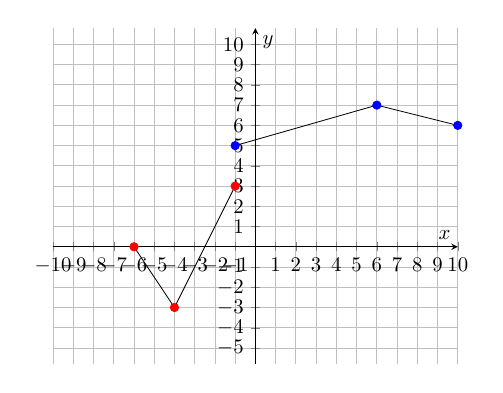
\begin{tikzpicture}[scale=.75]
		\begin{axis}[
			scatter/classes={f={draw=red,fill=red},g={draw=blue,fill=blue}},
			axis y line*=left,
			axis x line*=bottom,
			grid=both,
			ymin=-5,
			xmin=-10,
			ymax=10,
			xmax=10,
			axis equal,
			axis lines=middle,
			xlabel=$x$,
			ylabel=$y$,
			xtick distance= 1, ytick distance = 1
		]
		\addplot[scatter,scatter src=explicit symbolic]
			table[meta=label] {
				x y label
				-6 0 f
				-4 -3 f
				-1 3 f
				
				-1 5 g
				6 7 g
				10 6 g
			};
		\end{axis}
	\end{tikzpicture}\\
	To write the function $g(x)$ in the form $g(x)=af(b(x-c))+d$, we have to solve for all 4 of the variables, with 4 equations from the graph. We can know which point corresponds to which point because each segment will have the same proportions. Therefore, we can use these four equations (there are other possibilities): \[\]
	\subsubsection{Domain and Range}
	After transformations, the domain and range may be changed. The mapping formulas can be used to calculate the new ones.\\
	For example: A function with domain $D=(-1,3]$ and range $R=[2,\infty)$ is transformed into a new function $g(x)=-2f(2x-3)+4$. $a=-2$, $b=2$, $c=\frac{3}{2}$, $d=4$. The domain would be shifted to $\left(\frac{-1}{2}+\frac{3}{2}, \frac{3}{2}+\frac{3}{2}\right]=(1,3]$ and the range would be shifted to $\left[-2(2)+4, -2(\infty)+4\right)=[0, -\infty)$
	\subsection{Inverse Relations}
	\subsubsection{Inverse Relation}
	For any relation there is an inverse relation obtained by switching the $x$ and $y$ values for all the elements of the original relation. The inverse relation of a relation $r$ is denoted by $r^{-1}$. A 1:1 function is a function where the inverse is also a function; it passes both the vertical and horizontal line tests.\\
	The inverse relation of the relation $r=\{(1, 2), (1, 0), (-2, 1), (0, 2)\}$ is $r^{-1}=\{(2, 1), (0, 1), (1, -2), (2, 0)\}$
	\subsubsection{Symmetry}
	The graph of a relation and the graph of its inverse relation are symmetrical about the line $y=x$.
	%TODO: graph
	\subsubsection{Corresponding Key Points}
	A point $P(x, y)$ on the relation $r$ corresponds to the point $P'(y, x)$ on the inverse relation $r^{-1}$. The points $P$ and $P'$ are symmetrical about the line $y=x$.
	%TODO: graph
	\subsubsection{Domain and Range}
	The domain of the inverse relation $r^{-1}$ is the same as the range of the range of the relation $r$; $D_{r^{-1}}=R_r$. The range of the inverse relation $r^{-1}$ is the same as the domain of the range of the relation $r$; $R_{r^{-1}}=D_r$.\\
	A relation $r$ is given by the following mapping diagram:\\
	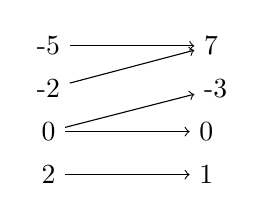
\begin{tikzpicture}[scale=.5]
		\node (n5) {-5};
		\node[below=2pt of n5] (n2) {-2};
		\node[below=2pt of n2] (o) {0};
		\node[below=2pt of o] (p2) {2};
	
		\node[right=45pt of n5] (p7) {7};
		\node[right=45pt of n2] (n3) {-3};
		\node[right=45pt of o] (o2) {0};
		\node[right=45pt of p2] (p1) {1};
	
		\draw[->] (n5) -- (p7);
		\draw[->] (n2) -- (p7);
		\draw[->] (o) -- (n3);
		\draw[->] (o) -- (o2);
		\draw[->] (p2) -- (p1);
	\end{tikzpicture}
	The domain of $r$ is $D={-5, -2, 0, 2}$ and the range is $R={-3, 0, 1, 7}$.
	The domain of $r^{-1}$ is $D={-3, 0, 1, 7}$ and the range is $R={-5, -2, 0, 2}$.
	\subsubsection{Inverse Relation of a Function}
	Any function is a relation. So, any function $f$ has an inverse relation $f^{-1}$.
\end{document}